
Though well-designed SPARQL is a fragment that covers a lot of practical SPARQL
queries, (50\% of the queries over DBpedia that use the
OPT-operator~\cite{Picalausa})
many practical queries are not well designed and need to be analyzed. 
Kaminski and Kostylev found another
interesting fragment of SPARQL called weakly well-designed fragment~\cite{kaminski_bwd}. This
fragment captures 99\% of the queries over DBPedia that use the OPT-operator. 
There are mainly two use cases of queries that are not well-designed but used in
practice.
\begin{enumerate}
	\item The first practical use of non well-designed patterns are the so called
		preference patterns:
		Consider the following example:
		\begin{example}[Preference Pattern~\cite{kaminski_bwd}]\label{prefpattern}
			\begin{align*}
				P_1 =	\SELECT x, y  \WHERE ((x,rdf:type,foaf:person)\\ \OPT (x,foaf:name,y))\\
				\OPT (x,v\_card:name,y)
			\end{align*}
		\end{example}
		It is obvious that the pattern $P$ in Example~\ref{prefpattern} 
		is not well-designed because variable
		$y$ does occur in two unrelated OPT parts of $P$. The
		intuitive meaning might seem unclear at the first moment, 
		but looking at the semantics of OPT sheds light on it: If the first OPT-operator
		does not bind the variable $y$ through the triple $(x, foaf:name, y)$ 
		and only then, $y$ is bound through the triple $(x, v\_card:name, y)$.
		This could be used when we have two relations, in this case $foaf:name$
		and $v\_card:name$, which connect a name to an identifier but we prefer
		the relation $foaf:name$ over $v\_card:name$.

	\item The second practical use of non well-designed patterns are top level
		FILTER expressions. Again for this usage consider the following query:
		\begin{example}[Top level
			Filter~\cite{kaminski_bwd}]\label{toplevelfilter}
			\begin{align*}
				P_2 = \SELECT x,y \WHERE ((x,rdf:type,foaf:person)\\ \OPT (x,
				foaf:name,y))\\ 
				\FILTER(\neg bound(y) \lor \neg(y = Ana)).
			\end{align*}
		\end{example}
		The query $P_2$ again is not well-designed because the FILTER constraint
		mentions the variable $y$, which occurs only in the optional
		part. The practical intention of the query is to filter for people
		where the name is not 'Ana' or do not have a name but an identifier
		bound by variable $x$.
\end{enumerate}

To capture the two use-cases mentioned in
Example~\ref{prefpattern} and Example~\ref{toplevelfilter}, well-designed SPARQL is extended to weakly well-designed SPARQL.
This new fragment subsumes well-designed queries and it was shown in~\cite{kaminski_bwd} 
that the fragment has the same complexity 
of query evaluation as well-designed queries. 
Also, $99\%$ of the practical queries over DBPedia containing OPT are now captured by a 
fragment which is well designed and thus efficient to evaluate.

\begin{definition}[Weakly well-designed patterns~\cite{kaminski_bwd}]
	A pattern $P$ is weakly well-designed (wwd-pattern) if each occurrence $i$
	of an OPT-subpattern  $(P_1\OPT P_2)$ variables in $vars(P_2) \backslash
	vars(P_1)$ appear outside $i$ only in
	\begin{itemize}
		\item subpatterns whose occurrences are dominated by $i$, and
		\item constraints of top-level occurrences of FILTER-patterns.
	\end{itemize}
\end{definition}
Checking if a pattern is wwd is very easy computationally:
\begin{proposition}[\cite{kaminski_bwd}]
	Checking whether a pattern $P$ belongs to the fragment $P_{wwd}$ can be done
	in time $O(|P|^2)$, where $|P|$ is the length of the string representation
	of $P$.
\end{proposition}
\begin{proofidea}
	In a simple recursive procedure, the top-level occurrences of filters are
	removed.  Then in yet another recursive procedure  the first condition of
	weakly well-designed patterns is checked. 
\end{proofidea}

\section{OPT-FILTER-Normal Form and Constraint Pattern Trees}
A convenience of using wd-patterns is being able to convert them to the so-called
OPT-normal form. In the OPT-normal form, all AND- and FILTER- subpatterns are
OPT-free and most importantly the pattern can then be naturally represented as a
tree. The resulting tree can be used to visualize how to evaluate and optimize
the original pattern~\cite{letelier2013static, pichler2014containment}. The tree
notation can be generalised to wwd-patterns.

\begin{definition}[OPT-FILTER-normal form~\cite{kaminski_bwd}]\label{ofnf}
	A pattern $P$ is in OPT-FILTER-normal form (or OF-normal form)
	if the following grammer can be tested positively:
	\begin{align*}
		&P ::=  F \mid (P \FILTER R) \mid (P \OPT S), \qquad S::= F\mid(S \OPT S),\\ 
	 &F ::=(B \FILTER R)
	\end{align*}
	where $B$ ranges over triple patterns and $R$ over filter
	constraints.
\end{definition}
As we can see from Definition~\ref{ofnf}, each triple pattern has a FILTER expression. 
This is no restriction because one can easily insert a dummy FILTER expression 
by letting $R = \top$. The basic patterns with FILTER expressions form the bottom layer.
On top of the bottom layer there is a combination of OPT and FILTER.
The layers cause that each occurrence of a FILTER-pattern in
the top layer is top-level. The normal form is AND-free: all conjunctions are
expressed via a set of triple patterns.

\begin{definition}[Constraint pattern tree
	(CPT)~\cite{kaminski_bwd}]\label{defcpt}
	A constraint pattern tree (CPT) $T(P)$ of a pattern $P$ in OF-normal form is
	the directed ordered labelled rooted tree, which can be recursively
	constructed as follows:
	\begin{enumerate}	
		\item if $B$ is a set of triple patterns then $T(B \FILTER R)$ is a single node
			$v$ labelled by the pair $(B,R)$;
		\item if $P'$ is not a set of triple patterns then $T(P' \FILTER R)$ is obtained
			by adding a special node labelled by $R$ as the last child of the
			root of $T(P')$;
		\item $T(P_1 \OPT P_2)$ is the tree obtained from $T(P_1)$ and $T(P_2)$
			by adding the root of $T(P_2)$ as the last child of the root of
			$T(P_1)$.
	\end{enumerate}
\end{definition}
Looking at Definition~\ref{defcpt} one can see the similarity of CPTs and
patterns in OF-normal form: A CPT displays the semantic structure of OPT and FILTER nesting.
The next step is to prove that every wwd-pattern can be converted to OF-normal
form and can be represented by a CPT, analogously to wd-patterns, which can be
transformed into  OPT-normal form and thus pattern trees. 
Towards this goal, the following equivalence is needed:
\begin{proposition}[\cite{kaminski_bwd}]
	Let $P_1,P_2,P_3$ be patterns and $R$ a filter constraint such that
	$vars(P_2) \cap vars(P_3) \subseteq vars(P_1)$ and $vars(P_2) \cap vars(R)
	\subseteq vars(P_1)$. Then the following equivalences hold:
	\begin{align*}
		(P_1 \OPT P_2) \AND P_3 \equiv (P_1 \AND P_3) \OPT P_2,\\
		(P_1 \OPT P_2) \FILTER R \equiv (P_1 \FILTER R) OPT P_2.
	\end{align*}
\end{proposition}
Using the two equivalences we can achieve our goal stated in
Proposition~\ref{wwdtoofnf}.

\begin{proposition}[\cite{kaminski_bwd}]\label{wwdtoofnf}
	Each wwd-pattern $P$ is equivalent to a wwd-pattern in $OF$-normal form of
	size $O(|P|)$.
\end{proposition}

Let $\prec$ be a relation which contains the topological sorting of the nodes in
$T(P)$ computed by a depth first search traversal. $v \prec u$ holds if $v$ is visited before
$u$ in the search process. Assuming such a relation $\prec$, Proposition~\ref{charwdcpt} 
provides a condition to decide whether a pattern is weakly well-designed looking
at its CPT.

\begin{proposition}[\cite{kaminski_bwd}]\label{charwdcpt}
	A pattern $P$ in OF-normal form is weakly well-designed iff. for each edge
	$(v,u)$ in its CPT $T(P)$ every variable $x \in vars(u) \backslash vars(v)$
	occurs only in nodes $w$ such that $v \prec w$. The pattern is well-designed
	iff. for every variable $x$ in $P$ the set of all nodes $v$ in $T(P)$ with
	$x \in vars(v)$ is connected.
\end{proposition}

Kaminski and Kostylev found a unique property, which applies only for
wwd-patterns: Each wwd-pattern is semantically equivalent to a pattern whose corresponding
CPT has depth one.
\begin{definition}[\cite{kaminski_bwd}]
	A pattern $P$ is in depth-one normal form if it has the structure
	\begin{align*}
		(\cdots((B \ op_1 \ S_1) \ op_2 \ S_2) \cdots)\ op_n \ S_n,
	\end{align*}
	where $B$ is a set of triple patterns and each $op_i S_i, 1 \leq i \leq n$ is either
	$\OPT (B_i \FILTER R_i)$ with $B_i$ a basic pattern and $R_i$ a filter
	constraint, or just FILTER $R_i$.
\end{definition}

Towards our goal to show that every wwd-pattern can be brought to the depth-one
normal form the following equivalence can be used.
\begin{proposition}[\cite{kaminski_bwd}]\label{equivdep1}
	For patterns $P_1, P_2,P_3$ with $vars(P_1) \cap vars(P_3) \subseteq
	vars(P_2)$ it holds that 
	\begin{align*}
		P_1 \OPT (P_2 \OPT P_3) \equiv (P_1 \OPT P_2) \OPT (P_2 \AND P_3).
	\end{align*}
\end{proposition}

\bigskip\noindent OPT operators in pattern can be nested in two different ways:
\begin{enumerate}
	\item $(P_1 \OPT (P_2 \OPT P_3))$ (OPT-R)
	\item $((P_1 \OPT P_2) \OPT P_3)$ (OPT-L)
\end{enumerate}
When we then use CPTs to display this patterns using triple patterns we get the following result:

\begin{figure}(1) 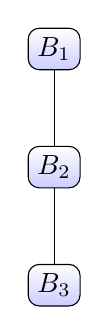
\begin{tikzpicture}[sibling distance=10em,
		every node/.style = {shape=rectangle, rounded corners,
			draw, align=center,
top color=white, bottom color=blue!20}]]
\node {$B_1$}
child { node {$B_2$} 
child { node {$B_3$} }};
\end{tikzpicture}
\hspace{5cm}
(2) 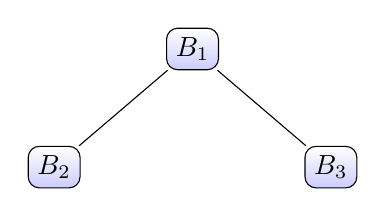
\begin{tikzpicture}[sibling distance=10em,
		every node/.style = {shape=rectangle, rounded corners,
			draw, align=center,
top color=white, bottom color=blue!20}]]
\node {$B_1$}
child { node {$B_2$} }
child { node {$B_3$} };
\end{tikzpicture}
\caption{(1) is the CPT of $(B_1 \OPT (B_2 \OPT B_3))$ and 
(2) the CPT of $((B_1 \OPT B_2) \OPT B_3)$}
\end{figure}\label{optrl}


Using the equivalence from left to right keeps the pattern weak well-designed and
transforms a weakly well-designed OPT nesting of type (OPT-R) to a nesting type
(OPT-L). Looking at the Figure~\ref{optrl} we can see that this step reduces the depth by one.
\begin{corollary}[\cite{kaminski_bwd}]
	Every wwd-pattern is equivalent to a wwd-pattern in depth-one normal form.
\end{corollary}
The regular structure of the depth-one normal form might prove attractive in
practice but using the equivalence results in an exponential blowup in the size
of the pattern. This can be seen in Proposition~\ref{equivdep1}: $P_2$ gets
copied twice in every application of the equivalence.

\section{Evaluation of wwd-Patterns}
The next step is to look at the complexity of the evaluation problem for
wwd-patterns and the extensions with union and projection. The goal is to show
that in all three cases complexity doesn't change in comparison to wd-patterns.
Consider first the formal evaluation problem for a given SPARQL fragment.
$\mathcal{L}$:
\begin{framed}\noindent \textbf{EVAL($\mathcal{L}$)}\\
	\textbf{INPUT:} Graph $G$, query $Q \in  \mathcal{L}$ and a mapping $\mu$.\\
	\textbf{QUESTION:} Is $\mu$ in $\ll Q \rr_G$.
\end{framed}
The fragment of general SPARQL graph patterns is denoted with $\u$ and it is a
well known result that $EVAL(\u)$ is PSPACE-complete~\cite{perez2009semantics}.
For the fragment of general queries extended with projection (i.e., $\s$)
it was shown that $EVAL(\s)$) is PSPACE-complete~\cite{letelier2013static}.
Considering now the fragment of wd-patterns, we know that the evaluation problem
is coNP-complete~\cite{letelier2013static} using the following algorithm:
Given a wd-Pattern $P$ in OPT-normal form, a graph $G$ and a mapping $\mu$.
\begin{enumerate}
	\item Look for a subtree $T_s$ of $T(P)$ including the root of $T(P)$ where the
		variables of the triples in $T_s$ are equal to the variables in $dom(\mu)$. 
		When we now use the mapping $\mu$ on all the triples, the triples must
		be in the graph $G$. This is doable in polynomial time. If such a $T_s$
		exists, $T_s$ witnesses	that $\mu$ is at least part of a solution in
		$G$.
	\item The second step is to check if the subtree $T_s$ is maximal. If we can
		extend $T_s$ with a node in $T(P)\backslash T_s$ and the mapping $\mu$ maps
		all the triples into $G$, the subtree $T_s$ was not maximal. There are
		linearly many nodes to check and each check can be performed in $coNP$.
		Resulting in an overall runtime of $coNP$.
\end{enumerate}
Similar to this algorithm, an algorithm for wwd-patterns exists. 
We first define the potential partial solutions. 
We know from the previous section that we can transform any wwd-pattern $P$ to a
pattern in OF-normal form. This pattern $P'$ in OF-normal corresponds to some
CPT. An $r$-subtree of $T(P')$ is a subtree containing the root of $T(P')$ and
all its special children. Every $r$-subtree obviously corresponds to some
wwd-pattern which is obtained by dropping the rightmost arguments of some
OPT-subpatterns.

\begin{definition}[\cite{kaminski_bwd}]
	Let $P$ be a wwd-pattern and $P'$ the corresponding pattern in OF-normal
	form.
	A mapping $\mu$ is a potential partial solution (or $pp$-solution for short)
	to a wwd-pattern $P$ over a graph $G$ if there is an r-subtree $T(P')$ of
	$T(P)$ such that $dom(\mu) = vars(P')$, $\mu(pat(P')) \subseteq G$ and $\mu
	\models R$ for the constraint $R$ of any ordinary node in $T(P')$.
\end{definition}

It could happen that several $r$-subtrees correspond to the same mapping $\mu$
for a pattern $P$ over $G$. We then take the union of all the nodes in exactly
those $r$-subtrees as they are a subtree as well. (They are all connected by the root). 
From this observation we can see that there exists a unique maximal r-subtree
corresponding to a mapping $\mu$ which we will from now on denote with
$T(P_\mu)$, as this subtree corresponds to a wwd-pattern $P_\mu$. The
big difference to partial solutions for wd-patterns is that not every pp-solution can be
extended to a real solution. A real solution may not only extend the domain of a pp-solution
with previously undefined variables but it might also extend $T(P_\mu)$ to a
child that is smaller in the order $\prec$ than some other node which was
already in $T(P_\mu)$. But this means that variables bindings might get
overriden. The next difference are non-well-designed top-level filters.
$pp$-solutions ignore top-level filters as it would be too restrictive as real
solutions do not satisfy them either. 

\begin{example}[\cite{kaminski_bwd}]
	Consider the graph $G = \{(1,a,1), (3,a,3)\}$ and the wwd-pattern:
	\begin{align*}
		P = (((x,a,1) \OPT (y,a,2)) \FILTER \neg bound(y)) \OPT (y,a,3).
	\end{align*}
	%	Consider now $T(P')$:\\
	%
	%	\begin{tikzpicture}[sibling distance=10em,
	%	 every node/.style = {shape=rectangle, rounded corners,
	%    draw, align=center,
	%    top color=white, bottom color=blue!20}]]
	%	\node {$(x,a,1),\top$}
	%	child { node {$(y,a,2),\top$} }
	%	child { node {$?(y,a,3),\top$}}
	%	child { node {$\neg bound(y)$}};
	%
	%	\end{tikzpicture}\\
	Obviously $\neg bound(y)$ is a top level filter and the whole pattern is
	not well designed as $y$ occurs in the top level filter.
	Also, the mapping $\mu = \{?X \mapsto 1, ?Y \mapsto 3\}$ is a solution in
	$\ll P \rr_G$, but we can see, that $\mu \not\models \neg bound(y)$.
\end{example}

The following characterisation takes care of the two difficulties and describes
solutions.
\begin{definition}[\cite{kaminski_bwd}]
	Given a wwd-pattern $P$, a node $v \in T(P)$, a graph $G$ and a
	$pp$-solution $\mu$ of $P$ over $G$, let $\mu_{|v}$ be the projection
	$\mu_{|X}$ of $\mu$ to the set $X$ of all variables appearing in nodes $u$
	of $T(P_\mu)$ such that $u \prec v$.
\end{definition}
$\mu_{|v}$ is in other words the mapping $T(P_\mu)$ until the node $v$ could be
considered in the order $\prec$ would traverse the tree $T(P)$.
\begin{lemma}[\cite{kaminski_bwd}]\label{lemsolwwd}
	A mapping $\mu$ is a solution to a wwd-pattern $P$ over a graph $G$ iff. 
	\begin{enumerate}
		\item $\mu$ is a pp-solution to $P$ over $G$.
		\item for any child $v$ of $T(P_\mu)$ labelled with $(B,R)$ there is no
			$\mu'$ such that $\mu_{|v} \sqsubset \mu'$, $\mu' \models R$, and
			$\mu'(B) \subseteq G$;
		\item $\mu_{|s} \models R$ for any special node $s$ in $T(P)$ labelled
			with $R$.
	\end{enumerate}
\end{lemma}
Intuitively we can conclude the following from the lemma: (1) is obvious and as
mentioned before, each solution needs to be a pp-solution of $P$ over $G$.
(2) makes sure that every node $v$ which is not added to $T(P_\mu)$ is not addable
to the tree ``until'' that node $v$ ``appears'' (i.e. in order of $\prec$) first. 
If it is addable it would mean,
that one could use the mapping bound up to node $v$ (looking at $\prec$, this is
$\mu_{|v}$) to create a new mapping
$\mu'$ which uses the node $v$. There are two ways of mapping $\mu'$
differently to the original mapping $\mu$: Either $dom(\mu)$ is extended, or
some variables are assigned differently because $\prec$ visits some node first
which contains the variable in a different triple resulting in a different
assignment.
(3) makes sure that the mapping fulfills the top-level filter at exactly the
timepoint where the traversal reaches the corresponding special node $s$, which
is denoted by $\mu_{|s}$.

\begin{theorem}[\cite{kaminski_bwd}]
	\textbf{EVAL($P_{wwd}$)} is coNP-complete.
\end{theorem}
\begin{proofidea}
	We can easily transform the characterisation in
	Lemma~\ref{lemsolwwd} to an	algorithm which is in coNP: 
	Compute the maximal tree for $\mu$, $T(P_\mu)$. This is doable in polynomial
	time. Now it remains to check that this tree is not extendable to linearly
	many of its children. As we then have to do a homomorphism check against
	$G$, this is in coNP. The checks for top-level filters are polynomial again.
\end{proofidea}

This result can easily be carried over to top level unions of wdd-patterns. The fragment
is called $\u_{wwd}$. The fragment where also projection is done over unions of
wdd-patterns is calles $\s_{wdd}$.

\begin{corollary}[\cite{kaminski_bwd}]
	\textbf{EVAL($\u_{wwd}$)} is coNP-complete and \textbf{EVAL($\s_{wwd}$)} is
	$\Sigma^P_2$-complete.
\end{corollary}
\begin{proofidea}
	The coNP-algorithm for $\u_{wwd}$ is easy to see, as we just apply the
	algorithm for  \textbf{EVAL($P_{wwd}$)} for every part of the top level UNION. And
	if the mapping $\mu$ is the solution for any of the patterns we return
	true. Hardness follows by the coNP-completeness of \textbf{EVAL($P_{wwd}$)}.
	It is a well known results that \textbf{EVAL($\s_{wd}$)} is $\Sigma^P_2$-complete,
	thus $\Sigma^P_2$-hardness of \textbf{EVAL($\s_{wdd}$)} follows. 
	For the $\Sigma^P_2$-membership of \textbf{EVAL($\s_{wdd}$)} apply the following algorithm:
	Guess the values of the existential variables and then call a coNP-oracle
	for $\u_{wwd}$ on the resulting mapping. This yields a $\Sigma^P_2$ algorithm.
\end{proofidea}

\section{Expressivity of wwd-Patterns and their Extensions}

\begin{definition}[Expressive power of languages]
	A language $\l_1$ has the same expressive power as language $\l_2$, denoted by
	$\l_1 \sim \l_2$, if for every query $Q_1 \in \l_1$ there is a query $Q_2 \in
	\l_2$ such that $Q_1 \equiv Q_2$ and for every query $Q_2 \in \l_2$ there is a
	query $Q_1 \in \l_1$ such that $Q_1 \equiv Q_2$ holds. 
	We write $\l_2 < \l_1$ if we can only find a query $Q_1 \in \l_1$ for every
	query $Q_2 \in \l_2$ but not vice versa.
\end{definition}
The goal for this section is to show the following results: 
\begin{enumerate}
	\item $P_{wd} < P_{wwd} <P$
	\item $\u_{wd} < \u_{wwd} < \u$
	\item $\s_{wwd} \sim \s$
\end{enumerate}
\begin{definition}
	A query $Q$ is weakly monotone if $\ll Q \rr_{G_1} \sqsubseteq \ll Q
	\rr_{G_2}$ for any two graphs $G_1$ and $G_2$ with $G_1 \subseteq G_2$.
	A fragment $\l$ is called weakly monotone if it contains only weakly
	monotone queries.
\end{definition}

Arenas and Perez showed in~\cite{arenas2011querying} that unlike $P$ the fragment
$P_{wd}$ is weakly monotone and hence $P_{wd} < P$.

\begin{theorem}[\cite{kaminski_bwd}]
	It holds that $P_{wd} < P_{wwd}$.
\end{theorem}
\begin{proof}
	We show the desired result by observing that $P_{wwd}$ is not weakly
	monotone.
	Consider the pattern
	\begin{align*}
		Q=((x,rdf:type,foaf:person) \OPT (x,foaf:name,y))\\
		\OPT (x,v\_card:name,y)
	\end{align*}
	and the two graphs
	\begin{align*}
		G_1 =& \{(P1,rdf:type,foaf:person) (P1, v\_card:name,Anastasia) \}
		\mbox{ and } \\
		G_2=& \{(P1,rdf:type,foaf:person), (P1, v\_card:name,Anastasia),\\
			&(P1, foaf:name, Ana) \}.
	\end{align*}
	Clearly $G_1 \subseteq G_2$. Let $\mu_1 = \{x \mapsto
	P1, y \mapsto Anastasia\}$ and let $\mu_2 = \{x \mapsto
	P1, y \mapsto Ana\}$. It is also clear considering that $Q$ is a priority
	pattern that $\mu_1 \in \ll Q \rr_{G_1}$ and  $\mu_2 \in \ll Q \rr_{G_2}$. But
	we cannot extend $\mu_1$ to $\mu_2$. Thus $\mu_1 \not\sqsubseteq \mu_2$ and
	thus $P_{wd} < P_{wwd}$ follows from the fact that $P_{wd}$ is weakly
	montone and the fact that $P_{wd} \subseteq P_{wwd}$.
\end{proof}

\begin{definition}[\cite{kaminski_bwd}]
	A query $Q$ is non-reducing if for any two graphs $G_1,G_2$ such that $G_1
	\subseteq G_2$ and any mapping $\mu_1 \in \ll Q \rr_{G_1}$, there is no
	$\mu_2 \in \ll Q \rr_{G_2}$ such that $\mu_2 \sqsubset \mu_1$ (i.e.$\mu_2
	\sqsubset \mu_1$ and $\mu_2 \neq \mu_1$).
	A fragment $\l$ is non-reducing if it contains only non-reducing queries.
\end{definition}

If a query is non-reducing it can happen that previously bound variable will get
unbound. It is easy to see that $wwd$-patterns are non-reducing as we can only
replace prior bindings but not erase them.

\begin{theorem}[\cite{kaminski_bwd}]
	It holds that $P_{wwd} < P$.
\end{theorem}
\begin{proof}
	Let 
	\begin{align*}
		P = (x, a, 1) \OPT ((y,a,2) \OPT(x,a,3)),
	\end{align*}
	\begin{align*}
		G_1 = \{(1,a,1),(2,a,2)\} \mbox{ and } G_2 = G_1 \cup \{(3,a,3)\}.
	\end{align*}
	Then $\mu_1 = \{x \mapsto 1, y \mapsto 2\}$ is the only mapping in $\ll
	P\rr_{G_1}$ while $\mu_2 = \{x \mapsto 1\}$ is the only mapping in $\ll P
	\rr_{G_2}$. Hence $\ll P \rr_{G_2} \sqsubset \ll P \rr_{G_1}$ even though
	$G_1 \subseteq G_2$. As we already mentioned $wwd$-patterns are non-reducing
	but this pattern is not non-reducing. Thus the desired result follows.
\end{proof}

The next step is to inspect the fragments $\u_{wd}$, $\u_{wwd}$ and $\u$.
It is easy to see that $\u_{wd}$ inherits weak monotonicity from
$P_{wd}$. Thus we can see that $\u_{wd} < \u_{wwd}$.
Unfortunately we cannot use non-reducibility as it doesn't propagate to unions.
Therefore a new condition is defined, namely extension-witnessing.

\begin{definition}
	A query $Q$ is extension-witnessing if for any two graphs $G_1 \subseteq
	G_2$ and mapping $\mu \in \ll Q \rr_{G_2}$ such that $\mu \not \in \ll Q
	\rr_{G_1}$ there is a triple $t$ in $Q$ such that $vars(t) \subseteq
	dom(\mu)$ and $\mu(t) \in G_2 \backslash G_1$. A fragment is
	extension-witnessing if all its queries are extension-witnessing.
\end{definition}

With this new condition, we can show that unions of wwd-patterns are
e-witnessing. 

\begin{theorem}[\cite{kaminski_bwd}]
	It holds that $\u_{wd} < \u_{wwd} < \u$.
\end{theorem}
\begin{proof}
	Again consider the counterexample from before:	
	\begin{align*}
		P = (x, a, 1) \OPT ((y,a,2) \OPT(x,a,3)),
	\end{align*}
	\begin{align*}
		G_1 = \{(1,a,1),(2,a,2)\} \mbox{ and } G_2 = G_1 \cup \{(3,a,3)\}.
	\end{align*}
	Then $\mu_1 = \{x \mapsto 1, y \mapsto 2\}$ is the only mapping in $\ll
	P\rr_{G_1}$ while $\mu_2 = \{x \mapsto 1\}$ is the only mapping in $\ll P
	\rr_{G_2}$.
	This is clearly not e-witnessing.
\end{proof}
Queries over unions of wwd-patterns are as expressive as full SPARQL.
\begin{theorem}[\cite{kaminski_bwd}]
	It holds that $\s_{wwd} \sim \s.$
\end{theorem}

\section{Static Analysis of wwd-Patterns}

\begin{theorem}[\cite{kaminski_bwd}]
	The problems \textbf{EQUIVALENCE($\l$)}, \textbf{CONTAINMENT($\l$)} and
	\textbf{SUBSUMPTION($\l$)} are $\Pi_2^P$-complete 
	for any $\l \in \{ P_{wwd}, U_{wwd} \}$.
\end{theorem}
\begin{proofidea}
	The membership result for \textbf{CONTAINMENT($\U_{wwd}$)} follows from the following
	counterexample property: 
	if $P \not\subseteq P'$ for some $P,P' \in \U_{wwd}$, then
	there is a witnessing mapping of size $O(|P| + |P'|)$.
	Consider the following $\Pi^P_2$-algorithm:
	Guess a mapping $\mu$ and a graph $G$ of linear size and check that $\mu
	\notin \ll P' \rr_G$ and then call a coNP oracle for checking if $\mu
	\in \ll P \rr_G$.
	Using this result we can show that \textbf{EQUIVALENCE($\u_{wwd}$)}  
	and \textbf{SUBSUMPTION($\u_{wwd}$)} are also in $\Pi^P_2$.
	The hardness proofs for \textbf{SUBSUMPTION($P_{wwd}$)} and\\
	\textbf{EQUIVALENCE($P_{wwd}$)} are by reduction from
	$\forall\exists3SAT$.\\
	\textbf{CONTAINMENT($P_{wwd}$)} is $\Pi^p_2$-hard by the results from~\cite{pichler2014containment}.
\end{proofidea}
